\section{What is \scalenetcdf file?}
In this section, \scalenetcdf file, which \scalelib directly reads from and writes in, is explained.
\scalelib employs \netcdf (network Common Data Format) as data file format.
\Netcdf is a software developed by Unidata (\url{http://www.unidata.ucar.edu/}),
and it enables us to generate files with self-describing and machine-independent data format;
for example, the former has a merit to describe variables along with their axis variables in a file and
the latter has a merit to treat data without worry which endian is used.
Based on the above virtue, \scalelib has particular conversion ( \scalenetcdf convention ).

\subsection{Global Attributes}
\scalenetcdf file contains information about data contained in the file,
such as those with regards to spatial decomposition as ``Global Attributes'' (Table \ref{table:netcdf_global_attrs}).
When the single file I/O is used (\nmitem{FILE_AGGREGATE}=.true. in \namelist{PARAM_FILE}),
the attributes of myrank, rankidx, and procsize are not output.

\begin{table}[bth]
\begin{center}
  \caption{Global attributes in \scalenetcdf file}
  \label{table:netcdf_global_attrs}
  \begin{tabularx}{150mm}{llX} \hline
    Name & description & remarks \\ \hline \hline
    title & brief description of data & value of \nmitem{History_TITLE} in \namelist{PARAM_HISTORY} \\
    source & name of the source software & value of \nmitem{History_SOURCE} in \namelist{PARAM_HISTORY}\\
    institution & data author & value of \nmitem{History_INSTITUTION} in \namelist{PARAM_HISTORY}\\
    myrank & rank id of MPI process & \verb|PRC_myrank| in the model \\
    rankidx & mapping index of the 2D decomposition & \verb|PRC_2Drank(PRC_myrank,1:2)| in the model \\
    procsize & number of the 2D decomposition & \verb|(/| \nmitem{PRC_NUM_X}, \nmitem{PRC_NUM_Y} \verb|/)| in the model \\ \hline
  \end{tabularx}
\end{center}
\end{table}

\noindent Refer Section \ref{sec:domain} for \nmitem{PRC_NUM_X, PRC_NUM_Y} and
Section \ref{sec:output} for \nmitem{History_TITLE, History_SOURCE, History_INSTITUTION}.


\subsection{Data in the halo region}

Whether the file 
contains the data in the halo region
depends on the type of file and its configuration.
Note that the halo region that we define here means the halo in the whole calculation region,
not the halo in each of local regions.

For the initial (or restart) and boundary data files, 
the halo data is contained if the lateral boundary conditions are not periodic 
(\nmitem{PRC_PERIODIC_X}, \nmitem{PRC_PERIODIC_Y} = .false. in \namelist{PARAM_PRC_CARTESC}) 
or the single file I/O is used (\nmitem{FILE_AGGREGATE}=.true. in \namelist{PARAM_FILE}),
otherwise it is not.

On the other hand,
for the history data file, 
the halo data is contained 
only when the lateral boundary conditions are not periodic
(\nmitem{PRC_PERIODIC_X}, \nmitem{PRC_PERIODIC_Y} = .false. in \namelist{PARAM_PRC_CARTESC})
and \nmitem{HIST_BND}=.true. in \namelist{PARAM_HIST},
otherwise it is not. Refer Section \ref{sec:output} for detail.

\subsection{Axis variables}
\scalenetcdf file contains axis data.
All the axis variables have 
``long\_name'' and ``units'' attributes,
which describe description and unit of the variable, respectively.
In addition, x, y, xh, and yh variables 
have attributes for the total number of grids in the whole domain ``size\_global'',
the start index in the total grid of data in the file ``start\_global'',
the number of the halo grids at the begin and end in the whole data ``halo\_global'',
and the number of the halo grids of data in the file ``halo\_local''.

Table \ref{table:netcdf_axes} shows list of the axis data.
The coordinate variables have their own dimension; their variable names are same as their dimension names.
The other axis variables use some dimensions of coordinate variables.
The lower-case variables are mainly used in the file, 
while the upper-case variables describe axes in simulation.
Figure \ref{fig:netcdfhorizontalcoordinate} and \ref{fig:netcdfverticalcoordinate} show 
the horizontal and vertical locations of coordinate variables,
respectively.
Refer to them with Table \ref{table:netcdf_axes} at the same time.

\begin{longtable}{l|l}
  \caption{Axis data in \scalenetcdf.}
  \label{table:netcdf_axes} \\ \hline
  \endfirsthead
  \multicolumn{2}{l}{\small\it Cont.} \\ \hline
%  & name & description \\ \hline \hline
  \endhead
  \hline
  \endfoot
  \multicolumn{2}{l}{Coordinate variables}\\ \hline
name & description \\ \hline \hline
\multicolumn{2}{c}{Common : Horizontal axis \& time}\\ \hline
x & full level position in x-direction of the data in the file \\
y & full level position in y-direction of the data in the file \\
xh & half level position in x-direction of the data in the file \\
yh & half level position in y-direction of the data in the file \\
time & time information \\ \hline
CX  & full level grid position in x-direction for the local region (inc. halo grids) \\
FX  & half level grid position in x-direction for the local region (inc. halo grids) \\
CDX & full level grid spacing  in x-direction (inc. halo grids) \\
FDX & half level grid spacing  in x-direction (inc. halo grids) \\
CY  & full level grid position in y-direction for the local region (inc. halo grids) \\
FY  & half level grid position in y-direction for the local region (inc. halo grids) \\
CDY & full level grid spacing  in y-direction (inc. halo grids) \\
FDY & half level grid spacing  in y-direction (inc. halo grids) \\
CXG & full level grid position in x-direction for the whole region (inc. halo grids) \\
FXG & half level grid position in x-direction for the whole region (inc. halo grids) \\
CYG & full level grid position in y-direction for the whole region (inc. halo grids) \\
FYG & half level grid position in y-direction for the whole region (inc. halo grids) \\ \hline
\multicolumn{2}{c}{Vertical axis : Atmosphere}\\ \hline
z   & full level position in z-direction in the file \\
zh  & half level position in z-direction in the file \\
CZ  & full level grid position in z-direction (inc. halo grids) \\
FZ  & half level grid position in z-direction (inc. halo grids) \\
CDZ & full level grid spacing  in z-direction (inc. halo grids) \\
FDZ & half level grid spacing  in z-direction (inc. halo grids) \\ \hline
\multicolumn{2}{c}{Vertical axis : Land}\\ \hline
lz   & full level position in z-direction of the land data in the file \\
lzh  & half level position in z-direction of the land data in the file \\
LCZ  & full level grid position in z-direction of the land model \\
LFZ  & half level grid position in z-direction of the land model \\
LCDZ & full level grid spacing in z-direction of the land model \\  \hline
\multicolumn{2}{c}{Vertical axis : Urban canopy}\\ \hline
uz   & full level position in z-direction in the file \\
uzh  & half level position in z-direction in the file \\
UCZ  & full level grid position in z-direction \\
UFZ  & half level grid position in z-direction \\
UCDZ & full level grid spacing in z-direction \\ \hline
 \hline
  \multicolumn{2}{l}{Other axis variables (1D)}\\ \hline
name  & description \\ \hline \hline
CBFZ  & buffer factor at CZ \\
FBFZ  & buffer factor at FZ \\
CBFX  & buffer factor at CX for the local region \\
FBFX  & buffer factor at FX for the local region \\
CBFY  & buffer factor at CY for the local region \\
FBFY  & buffer factor at FY for the local region \\
CBFXG & buffer factor at CXG for the whole region \\
FBFXG & buffer factor at FXG for the whole region \\
CBFYG & buffer factor at CYG for the whole region \\
FBFYG & buffer factor at FYG for the whole region \\
\hline
\multicolumn{2}{l}{Other axis variables (2D)}\\ \hline
name & description \\ \hline \hline
lon     & longitude at (y, x) \\
lon\_uy & longitude at (y, xh) \\
lon\_xv & longitude at (yh, x) \\
lon\_uv & longitude at (yh, xh) \\
lat     & latitude  at (y, x) \\
lat\_uy & latitude  at (y, xh) \\
lat\_xv & latitude  at (yh, x) \\
lat\_uv & latitude  at (yh, xh) \\
\hline
\multicolumn{2}{l}{Other axis variables (3D)}\\ \hline
name & description \\ \hline \hline
height      & heigth at (z, y, x)    in history file or at (y, x, z)    in restart/initial file\\
height\_xyw & height at (zh, y, x)   in history file or at (y, x, zh)   in restart/initial file\\
height\_xvz & height at (z, yh, x)   in history file or at (yh, x, z)   in restart/initial file\\
height\_uyz & height at (z, yh, xh)  in history file or at (hy, x, z)   in restart/initial file\\
height\_xvw & height at (zh, yh, x)  in history file or at (yh, x, zh)  in restart/initial file\\
height\_uyw & height at (zh, y, xh)  in history file or at (y, xh, zh)  in restart/initial file\\
height\_uvz & height at (z, yh, xh)  in history file or at (yh, xh, z)  in restart/initial file\\
height\_uvw & height at (zh, yh, xh) in history file or at (yh, xh, zh) in restart/initial file\\
\end{longtable}



\begin{figure}[tbh]
\begin{center}
  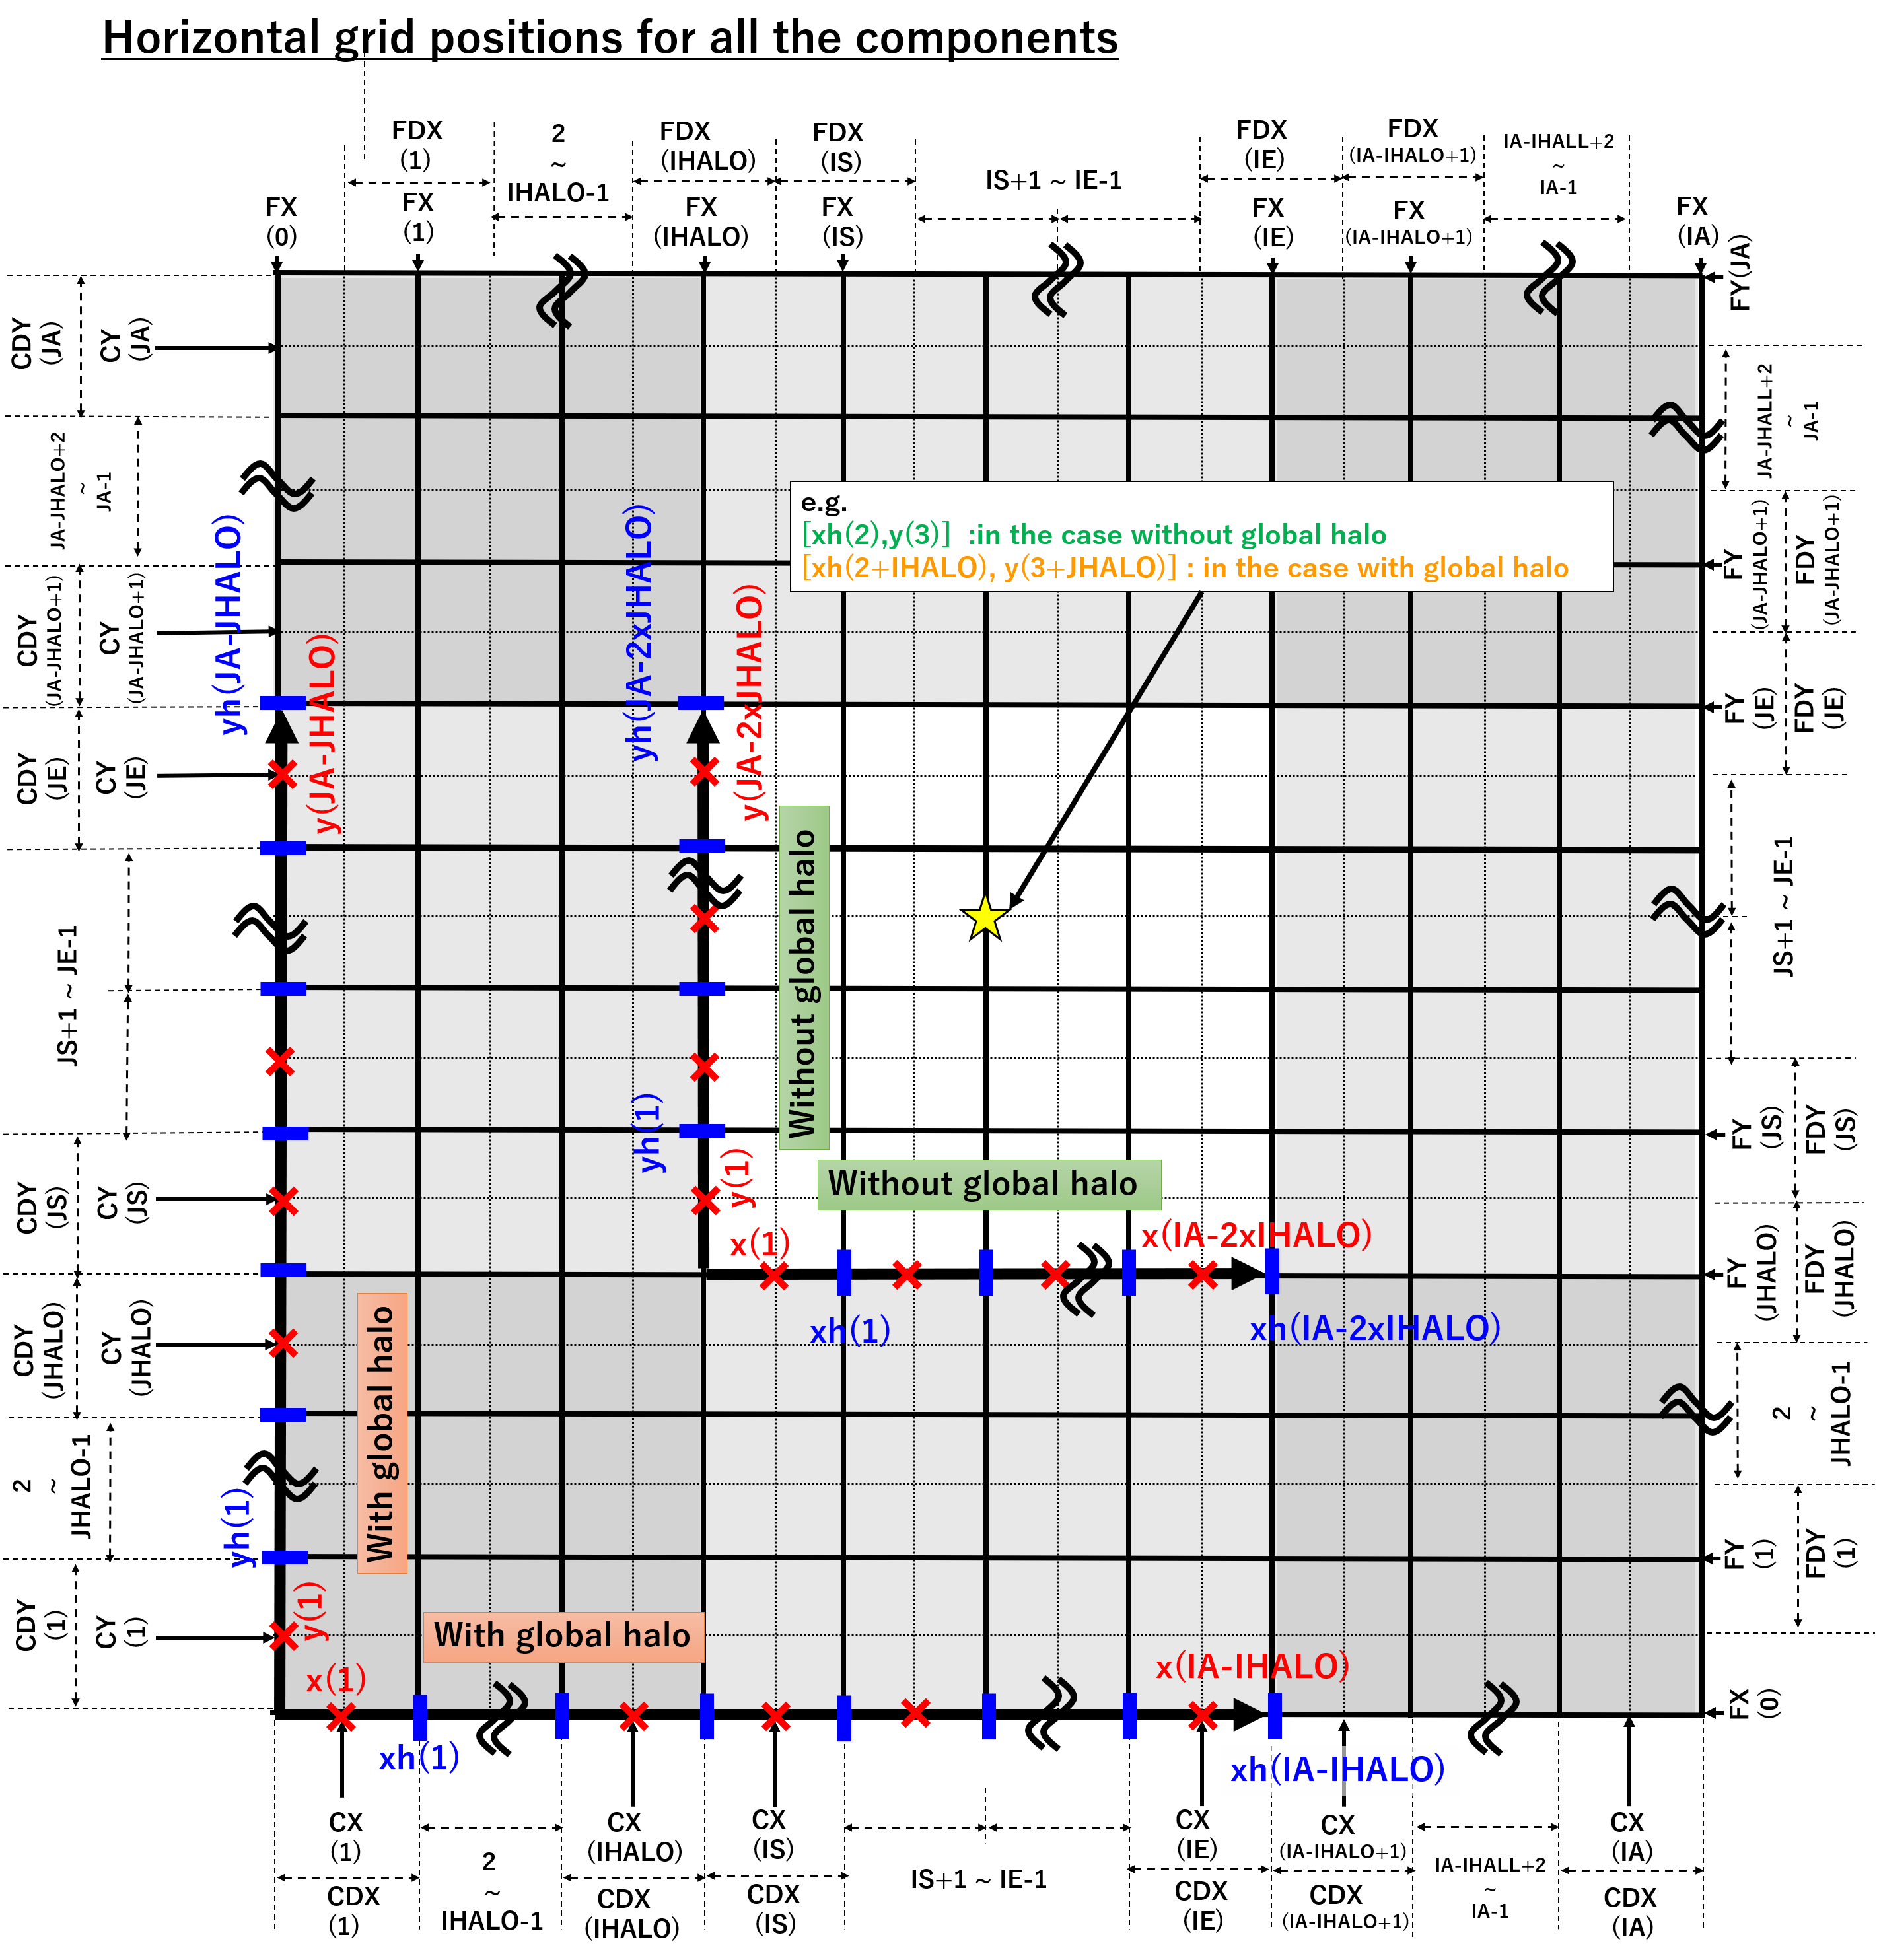
\includegraphics[width=1.0\hsize]{./figure/horizontal-coordinate-final2.png}\\
  \caption{Horizontal coordinate in \scalenetcdf file}
  \label{fig:netcdfhorizontalcoordinate}
\end{center}
\end{figure}
\begin{figure}[tbh]
\begin{center}
  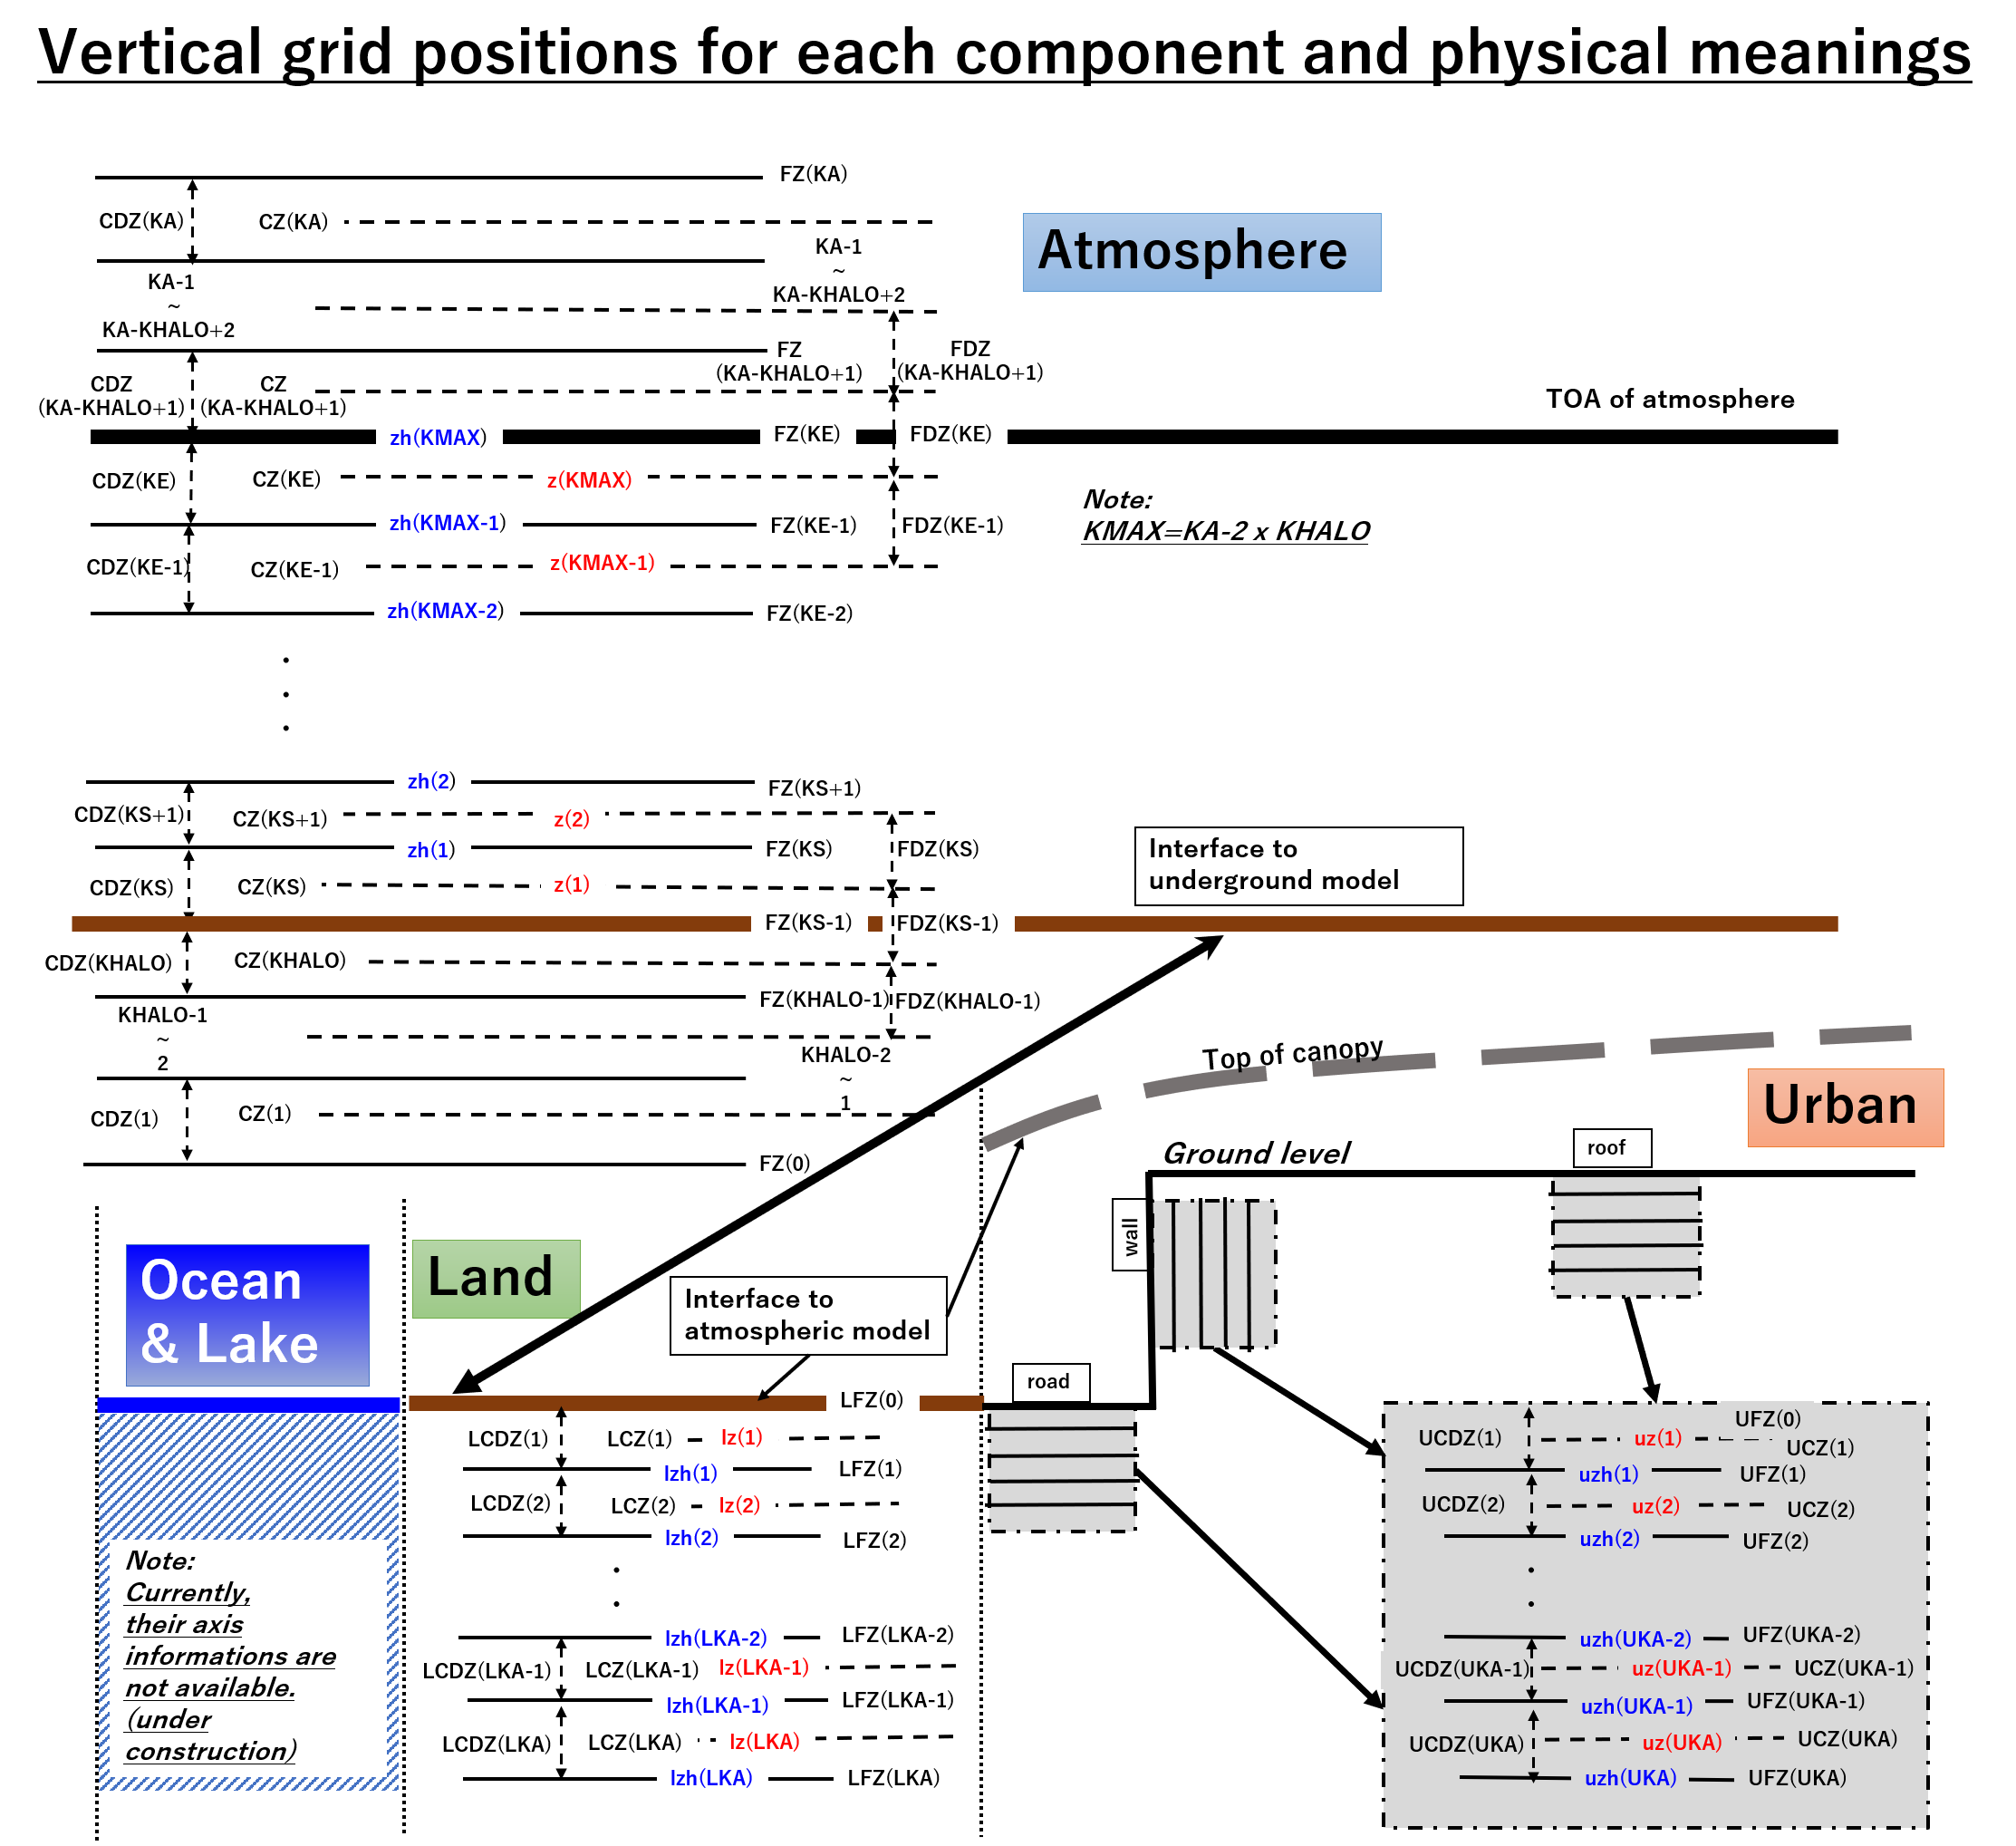
\includegraphics[width=1.0\hsize]{./figure/vertical_coordinate_final2.png}\\
  \caption{Horizontal coordinate in \scalenetcdf file}
  \label{fig:netcdfverticalcoordinate}
\end{center}
\end{figure}



\subsection{Data variables}
Data variables have attributes of the undefined value ``\_FillValue'' and 
the missing value ``missing\_value'' as well as ``long\_name'' and ``untis''.
Data structure in the initial (restart) data and boundary data files 
is identical to the array in the model, that is the z-x-y order.
On the other hand, it in the history data file is the x-y-z order.
This is true for 3D axis variables.
See also Table \ref{table:netcdf_axes}.

